%
% File acl2020.tex
%
%% Based on the style files for ACL 2020, which were
%% Based on the style files for ACL 2018, NAACL 2018/19, which were
%% Based on the style files for ACL-2015, with some improvements
%%  taken from the NAACL-2016 style
%% Based on the style files for ACL-2014, which were, in turn,
%% based on ACL-2013, ACL-2012, ACL-2011, ACL-2010, ACL-IJCNLP-2009,
%% EACL-2009, IJCNLP-2008...
%% Based on the style files for EACL 2006 by 
%%e.agirre@ehu.es or Sergi.Balari@uab.es
%% and that of ACL 08 by Joakim Nivre and Noah Smith

\documentclass[11pt,a4paper]{article}
\usepackage[hyperref]{acl2020}
\usepackage{times}
\usepackage{latexsym}
\usepackage{graphicx}
\usepackage{url}

\aclfinalcopy % Uncomment this line for the final submission
%\def\aclpaperid{***} %  Enter the acl Paper ID here

%\setlength\titlebox{5cm}
% You can expand the titlebox if you need extra space
% to show all the authors. Please do not make the titlebox
% smaller than 5cm (the original size); we will check this
% in the camera-ready version and ask you to change it back.

\newcommand\BibTeX{B{\sc ib}\TeX}

\title{Comparing Sarcasm Classification Across NLP Techniques}

\author{Jae Young Park \\
  DATASCI W266\\
  UC Berkeley \\
  School of Information \\
  {\tt jae\char`.park@berkeley.edu} \\}

\date{}

\begin{document}
\maketitle
\begin{abstract}
Sarcasm is a profoundly contextual phenomenon requiring shared knowledge. With recent advancements in Natural Language Processing, we are now closer than ever to detect linguistic phenomena that can are subtle but its cost to ignoring it are critical business usages. This paper attempts to test out a couple of practical ways to detect sarcasm.

Existing social media analysis systems are hampered by their inability to accurately detect and interpret figurative language. This is particularly relevant in domains like the social sciences and politics, in which the use of figurative communication devices such as sarcasm is common. With this in mind, we use data collected from Twitter to train and test out our models.

We provide some background on models that are typically used for sarcasm detection. A Naive Bayes model with out any context from the data is used to set a initial performance benchmark for the other models we will focus on: the Bidirectional CNN model and Text-To-Text Transfer Transformer(T5) model. 

Both models performed adequately, but the Bi-CNN did not beat our baseline, unlike the T5 model fine tuned with Huggingface's Transformers. This suggests that while the limitations in our sample size may be contributing to Bi-CNN model's performance, it has little effect on T5 model. This refutes the popular paradigm that the recently developed sophisticated models require more data to perform better than older models.

\end{abstract}

\section{Introduction}

Sarcasm is the use of words usually used to either mock or annoy someone, or for humorous purposes. Most noticeable in spoken word, sarcasm is mainly distinguished by the inflection with which it is spoken and is largely context-dependent.

The difficulty in recognition of sarcasm causes misunderstanding in everyday communication and poses problems to many NLP systems such as online review summarization systems, dialogue systems
or brand monitoring systems due to the failure of state of the art sentiment analysis systems to detect sarcastic comments.

The field of sentiment analysis can often be critical for business attempting to grow using customer testimony to present prospective customers with happy users experience with their products. A sarcastic message may, however, slip through the cracks, providing a scathing review hidden by heavy sarcasm that uses highly positive language. Sarcasm is also important in detecting toxic messages. Often times toxic messages are delivered using sarcastic comments. In both cases, it's possible to use the immediate context without having to rely on user-level data.

Some of the existing models rely heavily on information that may not be presented in the data itself (user information). That is, we must understand the user who's posting a message to understand if they are being sarcastic. Some algorithms even require knowledge of the target audience as well. Properly capturing this information however, may be unwieldy and perhaps even unethical. 

The first model we present uses convolutional neural networks that rely only on the context in which the message was posted. The context is defined in two ways. First, the prior tweet that the subject tweet is responding to. To do this, we collected the immediately prior tweet to which the twitter message of interest is responding to if they were responding to anything. The second definition of context is the given topic that the tweet is covering, which can be discovered by hashtags in Twitter.

The second model we present uses Text-To-Text Transfer Transformer created by Google AI, which states that T5 achieves state-of-the-art results on many NLP benchmarks while being flexible enough to be fine-tuned to a variety of important downstream tasks. Same as the first model, the context defined is provided to train the model. 

The paper relies on data scraped through Twitter to build our models, using the \#sarcasm, \#sarcastic, and \#s hashtags to label our training examples. We sample a set of popular hashtags as well to gather negative examples. For an even better performance on both models would require manual annotators to determine whether a given tweet is sarcastic. However, even this method proved to be challenging for many papers as even teams of expert annotators cannot completely be certain whether a message should be labeled as sarcastic.

\section{Background}

Historical experiments in this space have sourced data from social media channels like twitter, utilizing hashtags for labeling sarcasm (e.g. \#sarcasm, \#sarcastic, \#s, and \#not) as seen in the paper by Bamman and Smith. In the Bamman paper, logistic regression is used for classification by training the model with a combination of tweet, author and environmental features. From the paper by Amir et al, user-embeddings are used to help provide contextual features for their model.  Moreover, there have been more advanced approaches to detecting sarcasm by way of combining CNN, LSTM and DNN as seen in Ghosh and Veale. Additionally, some semi-supervised approaches are also used as done by Davidov et al. We compare the performances of these models against ours in the results section.

\section{Methods \& Data}
The objective of this paper is to predict whether a tweet is sarcastic or not. To measure the effectiveness of our methodologies, we will be using the average F1 score - which is a popular evaluation metric many authors discussed in the background section - between the two categories: sarcastic and non-sarcastic. 

Three methodologies are tested directly to detect whether a given tweet is sarcastic or not. the baseline model is a Naive Bayes model using a bag of words. The second model is a Bi-Convolutional Neural Network model, which uses the message of interest, and the message which is being responded to as the main set of features. The third model, which is the newest, implements Google's T5 model fine-tuned on our collected dataset.

The conventional 70-20-10 training-validation-test split is performed on our data, with additional testing data sourced from Twitter. 

\subsection{Data}
Referencing the Ghosh \& Veale and the Bannam \& Smith papers, we utilize functionality provided by twitter to access tweet data. Using the twitter streaming api for python, we collect sarcastic and non-sarcastic data.

As mentioned in Oprea \& Magdy paper, The most efficient way of collecting labeled data would be using the distant supervision method. To collect positive and negative examples of sarcasm we used self-declared labels of sarcasm with the following the \#sarcasm and \#sarcastic hashtags. An initial attempt also used the hashtag \#not, however the vast majority of tweets in this hashtag were not sarcastic, so they were removed from our analysis to get a cleaner look at the data. This shows the disadvantages of distant supervision, where we see the labels are incorrectly classified, making some of the data a semi labeled data that needs cleaning.

The tweet we collect from the stream are received in JSON objects. Features of the tweets that were of interest include user identification information, full text of the tweet including the hashtag labels, information connecting the tweet to any tweet and user that it is in reply to. We also see additional attributes such as language and geographical information for use. 

Since the context we work on in this problem involves people sending out the same message through various accounts through retweets, we choose not to remove a retweeted message as we can have access to the history of retweets in the context.

Since sarcasm is difficult to identify with inherent grounding issues, we aim to incorporate the previous tweet in the thread that our current data point is in response to. Although the objects obtained from twitter stream does have the user and status of the post it is in response to, it does not contain the previous status content itself.

\subsection{Data Exploration}
To ensure that the dataset is balanced, a check is done to see there are equal sample of sarcastic and non-sarcastic tweets in our training set. A total of about 19,160 tweets were used in our modeling processes.

Examples of sarcastic comments include:
 "@USER If the Antarctic ice sheets melt, the sea level would rise 216 feet. Nothing scary about that.", in response to a tweet on global warming.   
 
 "@USER @USER @USER Oatmilk is the best milk \#s". 
 
 The two examples shown above sums up the two majority cases of sarcastic tweets: the first case showing a seemingly positive response to an initial tweet that elicited a highly negative response, and the second cases where the tweet in subject immediately negates the general sentiment of the message within the hashtags. The hope is that our methodologies can detect these dramatic changes in sentiment and use them as a way to predict whether or not something may be satirical in nature.


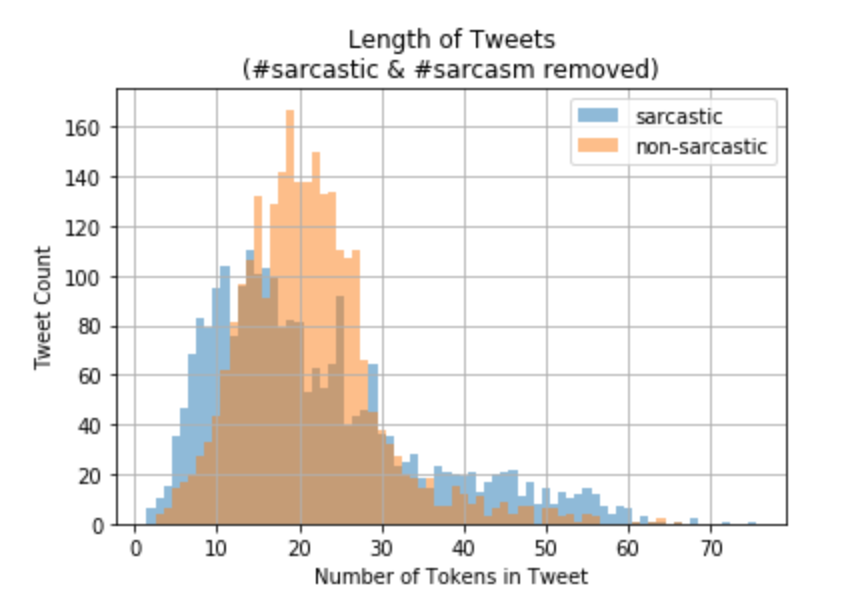
\includegraphics[width=75mm,scale=0.5]{token_histogram.png}

Also, By comparing the distribution of tweet length for sarcastic and non-sarcastic tweets, we see that there is a right skew in the sarcastic distribution. The higher number of tweets with fewer tokens for the sarcastic class may be indicative of there being more meaning grounded in context being referenced to - as we can see in the distribution of sarcastic tweets with context below. The tweet length for non-sarcastic tweets is centered around 20 tokens and seem to be more normally distributed as we might expect from given that we use a large number of popular topic hashtags to represent the general population. We can see above that, generally speaking we can contain the full content of a tweet distilled into a set of 60 tokens (over 95\% of tweets contained less than 60 tokens). For the CNN model, we assumed a length of 40 tokens, allowing us to pad short tweets and short context with a "PADDING" tokens to ensure consistent tweet length. Tweets longer than 40 tokens were truncated. This means that sarcastic tweets were more likely affected by this methodological decision. For the T5 model, we do not assume a length of the tokens, but only have a max input limit of 512, which probably leads to better performance of positive sarcasm detection.

Another point to review are the hashtag counts for both categories. 

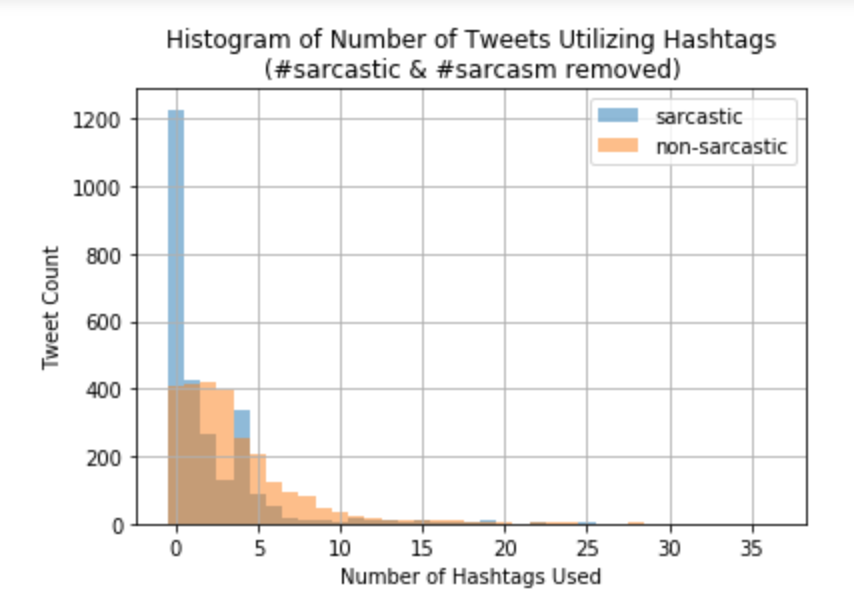
\includegraphics[width=75mm,scale=0.5]{hashtag_histogram.png}

We see that for sarcastic tweets there is a right-skewed in the distribution of number of hashtags used in a given tweet. This means that for any sarcastic tweets, we expect the user will be less likely to use additional tags to accompany the \#sarcasm, \#sarcastic, and \#s hashtags. In the non-sarcastic distribution there is less of a skew in the distribution with a median value around 4 hashtags in a tweet. We can see that in general, non sarcastic tweets are more likely to include hashtags for words other than the ones we used to sample our data. 

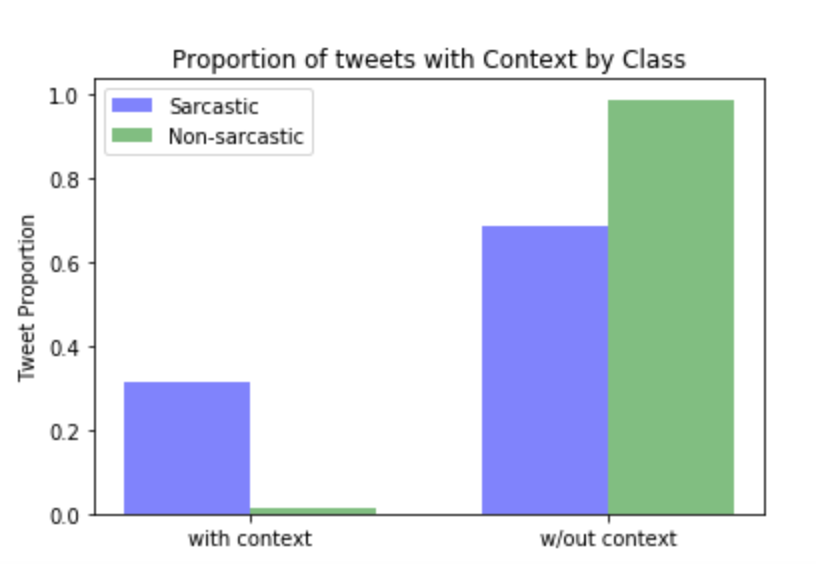
\includegraphics[width=75mm,scale=0.5]{context_proportion.png}

The bar chart above shows that both for sarcastic and non-sarcastic tweet have a larger proportion of tweets that are not in response to a preceding tweet in a message thread.  However, when looking at the left group of bars showing those proportions of the each of the two classes of tweets that have context, we see that there is a much higher percentage of sarcastic tweets with context than non-sarcastic tweets.

\subsection{Defining our Vocabulary}

Aside from utilizing Google's Colossal Clean Crawled Corpus (C4) that is used to pre-train our T5 model, the paper takes two main approaches to define the vocabulary. The key difference in the approach is the treatment of hashtags. In one hand, hashtags are tokenized as separate tokens. This allows us to capture additional context that may not be available in using only the prior tweet. Also, to confirm that this methodology helped improve accuracy of our model, we map all hashtags to a single token, which we named "HASHTAG". 

Under both methodologies, we tokenize all URLs as "LINK" tokens, retweet tags (including username attached to that retweet as "retweet", all remaining usernames as "USERS", and finally each digit in a number as DG. 

\subsection{Baseline - Multinomial Naive Bayes}
The baseline is constructed using a word count-based multinomial Naive Bayes bag of words model with Laplace smoothing. The bag of words is defined using the methodology described above. 
Through a series of testing the optimal alphas using cross-validation, 0.1 proved to be optimal for our data set.

\subsection{Bi-Convolutional Neural Network Model}

This model is implemented using an architecture proposed by Yin et. al. Two separate CNN processes run where one processes the context sentence and the other processes the tweet of interest. An embedding layer generates an embedding vector for each token in our vocabulary. This embedding layer is shared between the two CNN processes. We decide not to use pre-trained word vectors as we want to capture the dynamic nature of twitter tweets as well as generate word vectors for hashtags and emojis. 

Each set of word vectors is then concatenated together and is then passed through the convolutional layer. By padding our tweets, we effectively have what is a variation of the wide variation. This variation generates an embedding for the "PADDING" token instead of a 0 embedding. The convolution layer also allows for the sharing of the convolution weights across the two processes. Similar to Yin et. al, we use an average pooling layer that results in a tweet embedding vector of the same size as the word embedding vectors. The two resulting tweet vectors are concatenated together, and a logistic regression output layer is applied to the concatenated word vectors.

A diagram describing this procedure is below.

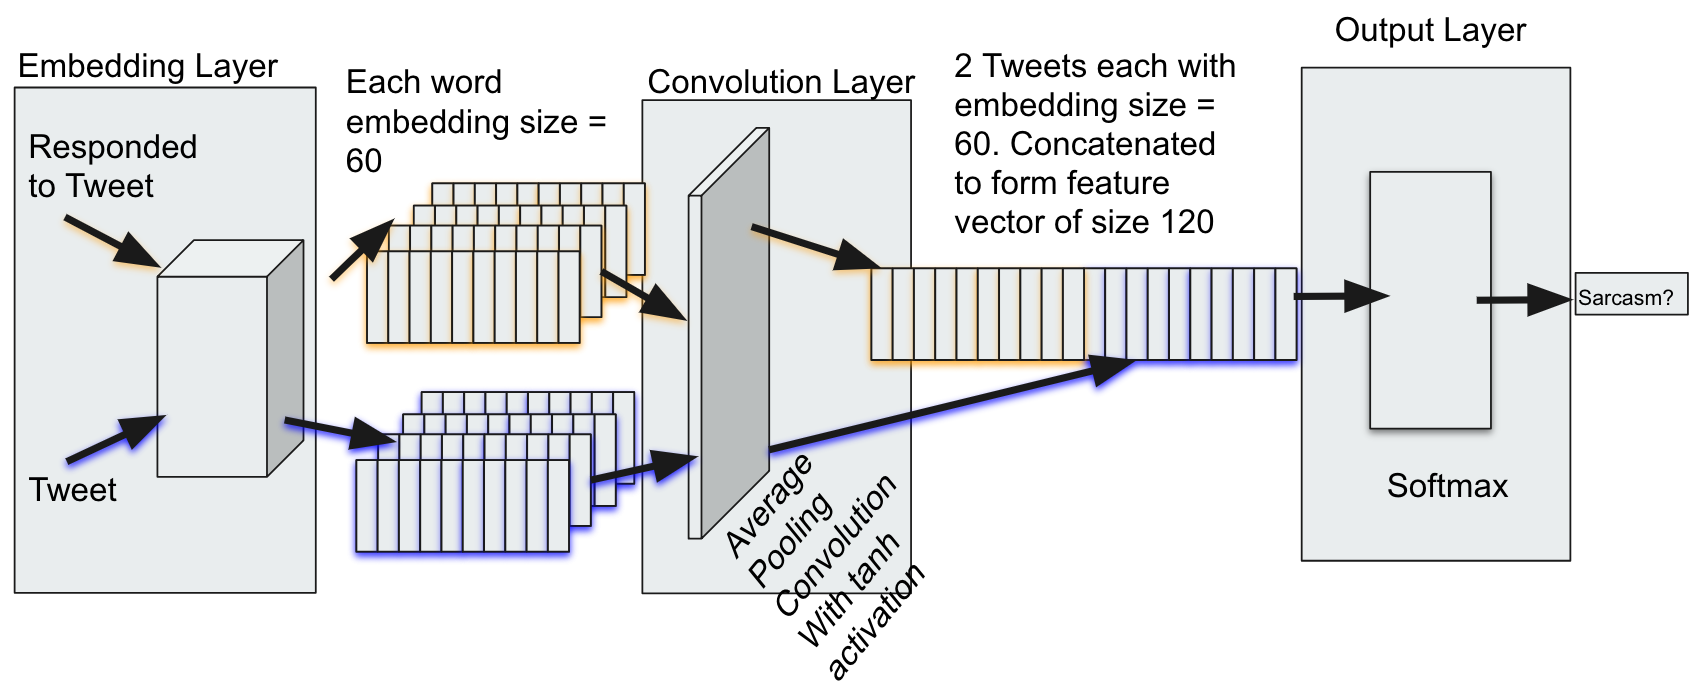
\includegraphics[width=75mm,scale=0.5]{bcnn.png}

The implementation of the algorithm that we rely on in this paper is using an embedding vector size of 60, a dropout keep probability of 40\%, a batch size of 200, using 10 epochs and no L2 regularization, which we determined using a series of cross validation tests.

\subsection{Fine-tuned T5 Model}

This model is implemented using an architecture proposed by Google AI's Text-To-Text Transfer Transformer. This is a Transformer based architecture that uses a text-to-text approach where every task – including translation, question answering, and classification – is cast as feeding the model text as input and training it to generate some target text. This allows for the reuse of the same model, loss function, hyper-parameters, etc. across our diverse set of tasks for any type of dataset with minimal change in code. This is essentially a Encoder-Decoder Transformer with some changes like applying Layer Normalization before a sub block, and then adding the initial input to the sub-block output - also known as pre-norm. Moreover, the model configuration is similar to BERT base. Compared to BERT, which has been the most likely used architecture model for NLP these recent years, adds a causal decoder to the bidirectional architecture and replaces the fill-in-the-blank close task with a mix of alternative pre-training tasks.

This paper uses the pytorch-lightning library for training with the help from the huggingface transformer library. This implementation of 5T also uses the batch size of 8 and gradient accumulation steps of 16, making the effective batch size as 128. 



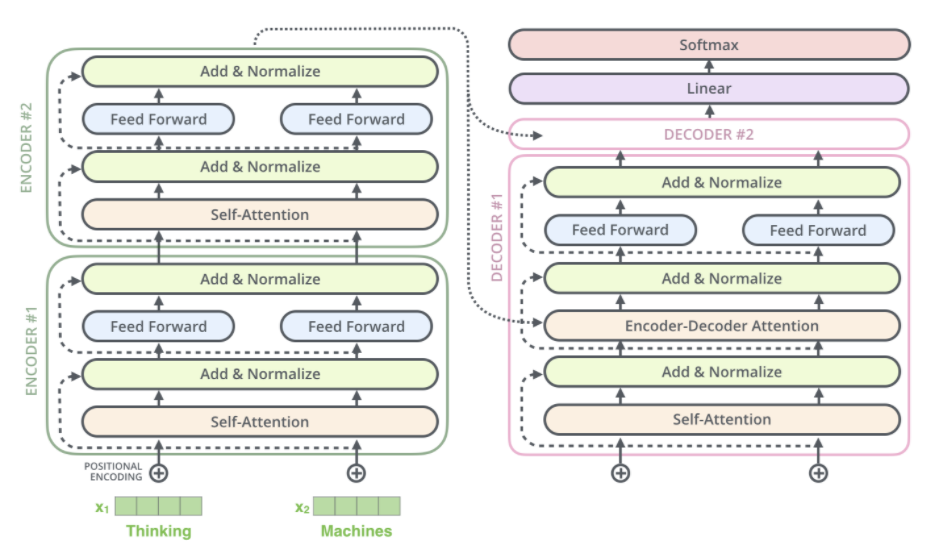
\includegraphics[width=75mm,scale=0.5]{T5_arch.png}


\section{Results and Error Analysis}

A comparison of the different models we built as well as the best models proposed by the authors discussed in the background research section can be seen below.

% \includegraphics[width=75mm,scale=0.5]{results.png}
\begin{center}
%  \begin{tabular}{|c{5em}|| c{1cm} c{1cm} c{1cm} c{1cm}|} 
 \resizebox{\columnwidth}{!}{\begin{tabular}{|c|| c c c c|}
 \hline
 Model & Recall & Precision & F1-Score & Accuracy \\ [0.5ex] 
 \hline\hline
 Davidov et. Al & 37.0\% & 79.8\% & 50.5\% & 90.6\% \\ 
 \hline
 Bamman and Smith. Al & & & & 81.2\% \\ 
 \hline
 Ghosh and Veale & 92.3\% & 91.9\% & 92.1\% & \\ 
 \hline
 Naive Bayes Hashtags & 93.1\% & 89.8\% & 91.3\% & 91.3\% \\
 \hline
 Naive Bayes No Hashtags & 87.8\% & 84.4\% & 86.3\% & 86.1\% \\
 \hline
 Bi-CNN Hashtags & 94.2\% & 84.3\% & 89.0\% & 88.4\% \\ 
 \hline
 Bi-CNN No Hashtags & 65.3\% & 93.4\% & 76.9\% & 80.5\% \\
 \hline
 Fine-tuned T5 & 92.8\% & 93.3\% & 93.4\% & \\ 
 \hline


\end{tabular}}
\end{center}

Surprisingly, the baseline Naive Bayes model outperforms most of the works presented by the authors described, including the Bi-CNN model. However, our fine-tuned T5 model outperforms every single model presented in this paper, showing an average f1-score of 93.4\%, and both 93\% on sarcastic and non-sarcastic test data.

To check for common errors, we randomly sample from the top tweets that the models incorrectly classified. One common error mostly present in all models is the classification of compliments. It seemed to consider compliments as sarcastic. Likely, what this shows is that compliments in twitter are rare, and when a compliment is seemingly made of someone, it is sarcastic. 

Also, as described in our data exploration section, non-sarcastic tweets were much more likely to heavily use hashtags. For this reason the models which mapped all hashtags to a single "HASHTAG" token were overconfident in tweets where a large number of hashtags were present in the tweet, an issue we attempted to remedy by mapping each hashtag to its own token.

\section{Conclusion}

In a sense, this paper marks the remarkable advancement of NLP techniques throughout the the recent years. We start with implementing the baseline multinomial Naive Bayes model with Laplace smoothing. This model resulted in surprisingly accurate predictions while also uncovering interesting phenomena within the sarcastic hashtags and emojis.

We then implement the  Bi-CNN model, which encodes sarcasm using two separate sentences, the tweet that our tweet of interest is responding to as well as the tweet of interest itself. This allows us to forego the use of user embeddings while still building context, without a significant loss of accuracy compared to the models described by other authors. One caveat of this methodology is that the data is likely heavily over-fitting to the context which we collected our non-sarcastic training data.

The final model that we implement is the fine-tuned T5 model, an encoder-decoder model pre-trained on a multi-task mixture of unsupervised and supervised tasks and for which each task is converted into a text-to-text format. With T5 Pre-trained on Colossal Clean Crawled Corpus, we were able to fine-tune the base model with our twitter dataset to achieve the highest performance metric amongst the models in this paper. Two directions of improvement with this model in the future would include an addition of a more expansive dataset that covers more than the 10 categories of interest in our dataset, and the use of ensemble learning approaches, both of which are not included in this paper due to time constraint.
\section{References}

Dmitry Davidov, Oren Tsur and Ari Rappoport. Semi-Supervised Recognition of Sarcastic Sentences
in Twitter and Amazon. In Proceedings of the Fourteenth Conference on Computational Natural Language Learning, pages 107–116, Uppsala, Sweden, 2010.
\\
\\
David Bamman and Noah A. Smith. Contextualized Sarcasm Detection on Twitter. Association for the Advancement of Artificial Intelligence, 2015.
\\
\\
Wenpeng Yin, Hinrich Schutze, Bing Xiang and Bowen Zhou. ABCNN: Attention-Based Convolutional Neural Network for Modeling Sentence Pairs. arXiv:1512.05193, 2016.
\\
\\
Silvio Amir, Byron C. Wallace, Hao Lyu, Paula Carvalho Mario and J. Silva. Modelling Context with User Embeddings for Sarcasm Detection in Social Media. arXiv:1607.00976v2, 2016.
\\
\\
Aniruddha Ghosh and Tony Veale. Fracking Sarcasm using Neural Network. Proceedings of NAACL-HLT 2016, pages 161–169, 2016.
\\
\\
Silviu Vlad Oprea and Walid Magdy. iSarcasm: A Dataset of Intended Sarcasm. Proceedings of the 58th Annual Meeting of the Association for Computational Linguistics, pages 1279–1289, 2020.
\\
\\
Debanjan Ghosh, Avijit Vajpayee and Smaranda Muresan. A Report on the 2020 Sarcasm Detection Shared Task. Proceedings of the Second Workshop on Figurative Language Processing, pages 1–11, 2020.
\\
\\
Colin Raffel, Noam Shazeer, Adam Roberts, Katherine Lee, Sharan Narang, Michael Matena, Yanqi Zhou, Wei Li and Peter J. Liu. Exploring the Limits of Transfer Learning with a Unified Text-to-Text Transformer. arXiv:1910.10683v3 [cs.LG], 2020.

\end{document}

\end{document}
